\documentclass[a4paper,11pt]{article}\usepackage[]{graphicx}\usepackage[]{xcolor}
% maxwidth is the original width if it is less than linewidth
% otherwise use linewidth (to make sure the graphics do not exceed the margin)
\makeatletter
\def\maxwidth{ %
  \ifdim\Gin@nat@width>\linewidth
    \linewidth
  \else
    \Gin@nat@width
  \fi
}
\makeatother

\definecolor{fgcolor}{rgb}{0.345, 0.345, 0.345}
\newcommand{\hlnum}[1]{\textcolor[rgb]{0.686,0.059,0.569}{#1}}%
\newcommand{\hlsng}[1]{\textcolor[rgb]{0.192,0.494,0.8}{#1}}%
\newcommand{\hlcom}[1]{\textcolor[rgb]{0.678,0.584,0.686}{\textit{#1}}}%
\newcommand{\hlopt}[1]{\textcolor[rgb]{0,0,0}{#1}}%
\newcommand{\hldef}[1]{\textcolor[rgb]{0.345,0.345,0.345}{#1}}%
\newcommand{\hlkwa}[1]{\textcolor[rgb]{0.161,0.373,0.58}{\textbf{#1}}}%
\newcommand{\hlkwb}[1]{\textcolor[rgb]{0.69,0.353,0.396}{#1}}%
\newcommand{\hlkwc}[1]{\textcolor[rgb]{0.333,0.667,0.333}{#1}}%
\newcommand{\hlkwd}[1]{\textcolor[rgb]{0.737,0.353,0.396}{\textbf{#1}}}%
\let\hlipl\hlkwb

\usepackage{framed}
\makeatletter
\newenvironment{kframe}{%
 \def\at@end@of@kframe{}%
 \ifinner\ifhmode%
  \def\at@end@of@kframe{\end{minipage}}%
  \begin{minipage}{\columnwidth}%
 \fi\fi%
 \def\FrameCommand##1{\hskip\@totalleftmargin \hskip-\fboxsep
 \colorbox{shadecolor}{##1}\hskip-\fboxsep
     % There is no \\@totalrightmargin, so:
     \hskip-\linewidth \hskip-\@totalleftmargin \hskip\columnwidth}%
 \MakeFramed {\advance\hsize-\width
   \@totalleftmargin\z@ \linewidth\hsize
   \@setminipage}}%
 {\par\unskip\endMakeFramed%
 \at@end@of@kframe}
\makeatother

\definecolor{shadecolor}{rgb}{.97, .97, .97}
\definecolor{messagecolor}{rgb}{0, 0, 0}
\definecolor{warningcolor}{rgb}{1, 0, 1}
\definecolor{errorcolor}{rgb}{1, 0, 0}
\newenvironment{knitrout}{}{} % an empty environment to be redefined in TeX

\usepackage{alltt}
\usepackage[onehalfspacing]{setspace}
\usepackage{hyperref}
\hypersetup{
    colorlinks = true, 
    citecolor = blue, 
    linkcolor = blue, 
    filecolor = blue, 
    urlcolor = blue
}
\newcommand{\code}[1]{\texttt{#1}}
\usepackage[margin=2.5cm]{geometry} 
\usepackage{float}
\usepackage{caption}
\captionsetup[table]{justification=justified, labelfont={bf}, singlelinecheck=false, font={normal, stretch=1}, format=plain, labelsep=newline, skip=2pt}
\captionsetup[figure]{justification=justified, labelfont={bf}, font={normal, stretch=1}, format=plain}

\usepackage{booktabs}
\usepackage{longtable}
\usepackage{array}
\usepackage{multirow}
\usepackage{wrapfig}
\usepackage{colortbl}
\usepackage{pdflscape}
\usepackage{tabu}
\usepackage{threeparttable}
\usepackage{threeparttablex}
\usepackage[normalem]{ulem}
\usepackage{makecell}
\usepackage{xcolor}

\author{P468}
\title{MSc Statistical Programming 2024}
\IfFileExists{upquote.sty}{\usepackage{upquote}}{}
\begin{document}

\maketitle



\section{U.K. House Prices}

\begin{enumerate}






\item In Figure \ref{fig:plot_price_countries}, we plot the average house price for the four nations: England, Northern Ireland, Scotland and Wales. We observe that the average house price is currently the highest in England, followed by Wales, Scotland and Northern Ireland. Besides that, when looking further back in time, we observe that this ordering has been relatively stable over time. One exception is maybe between 2000 and 2008. During this period, the average house prices in all four countries rose rapidly, but especially those in Northern Ireland. This led to a climax in the years before 2008, when the house prices in Norther Ireland were on average even larger than those in England. Interestingly, the apparent bubble in the Irish housing market collapsed in 2008, since the average house price declined drastically. This is also known as the Irish property bubble and marks the end of the so-called \textit{Celtic Tiger}.

\begin{knitrout}
\definecolor{shadecolor}{rgb}{0.969, 0.969, 0.969}\color{fgcolor}\begin{figure}[H]

{\centering 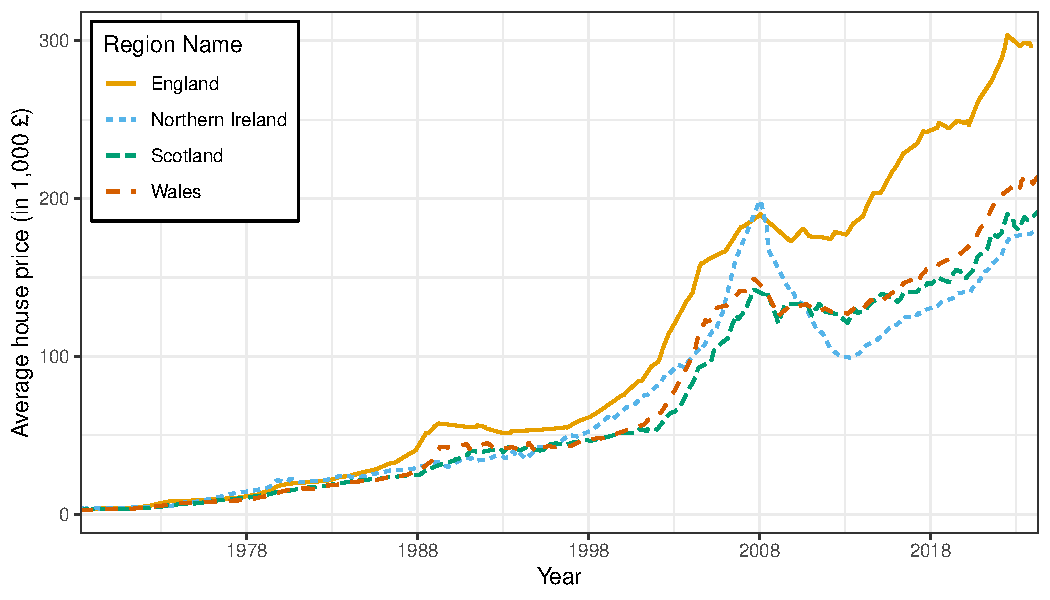
\includegraphics[width=0.8\linewidth]{figure/plot_price_countries-1} 

}

\caption[Average house price for England, Scotland, Wales, and Northern Ireland]{Average house price for England, Scotland, Wales, and Northern Ireland}\label{fig:plot_price_countries}
\end{figure}

\end{knitrout}






\item Moreover, we want to plot the average house prices for England and the four regions that have ``Cambridge" in the region name. We want to restrict the date range in the plot to only those dates for which England and Cambridge regional information are available. Table \ref{tab:table_cambridge} presents the four regions of Cambridge together with the first and last date for which the average house price is available in our sample. We observe that for all Cambridge regions the price series is available from 1995-01-01. For England, however, the first observation is already in 1968-04-01. The last observation for all regions is made at 2024-07-01. Furthermore, it can be shown that we do not have regions with missing price-observations between 1995-01-01 and 2024-07-01. Therefore, we restrict the plotting period to these dates. \par 

\begin{knitrout}
\definecolor{shadecolor}{rgb}{0.969, 0.969, 0.969}\color{fgcolor}\begin{table}[H] \captionsetup{margin = 105pt}
\centering
\caption{\label{tab:table_cambridge}The four regions of Cambridge together with the first and last date observed in our sample}
\centering
\begin{tabular}[t]{lll}
\toprule
Region Name & First date & Last date\\
\midrule
Cambridge & 1995-01-01 & 2024-07-01\\
Cambridgeshire & 1995-01-01 & 2024-07-01\\
East Cambridgeshire & 1995-01-01 & 2024-07-01\\
England & 1968-04-01 & 2024-07-01\\
South Cambridgeshire & 1995-01-01 & 2024-07-01\\
\bottomrule
\end{tabular}
\end{table} \captionsetup{margin = 105pt}

\end{knitrout}

Figure \ref{fig:plot_average_price_cambridge} plots the average house price for England and the four Cambridge regions. In general, we observe that the average house price in the Cambridge regions is higher than those in England since 1995. Especially the prices in Cambridge and Cambridgeshire are high relative to England, and this absolute difference seems to have grown over time. 

\begin{knitrout}
\definecolor{shadecolor}{rgb}{0.969, 0.969, 0.969}\color{fgcolor}\begin{figure}[H]

{\centering 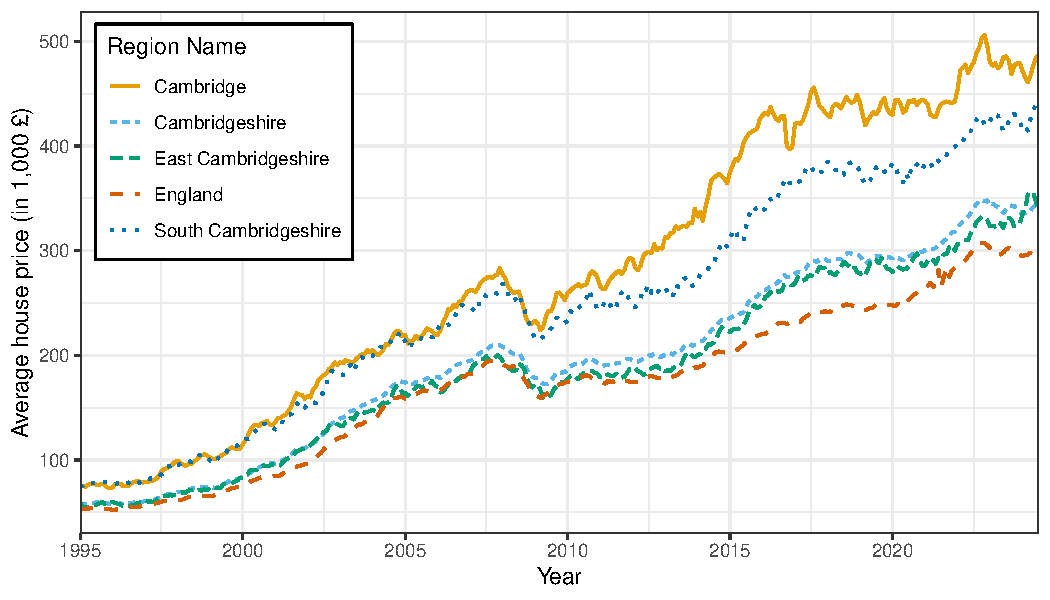
\includegraphics[width=0.8\linewidth]{figure/plot_average_price_cambridge-1} 

}

\caption[Average house price for England and the four regions of Cambridge]{Average house price for England and the four regions of Cambridge}\label{fig:plot_average_price_cambridge}
\end{figure}

\end{knitrout}




\item In this section, we determine the regions in England for which the average house price has been the highest over time. We define the regions in England as those for which the first character of the \code{Area\_Code} variable is ``E". Then, for each of those regions, we calculate the monthly ratio of the average house price for that region relative to the average price in England, where the observations are matched by date. By comparing the median of those ratios between regions, we get some idea of where in England the average house prices have been highest over time. 

\begin{knitrout}
\definecolor{shadecolor}{rgb}{0.969, 0.969, 0.969}\color{fgcolor}\begin{table}[H] \captionsetup{margin = 15pt}
\centering
\caption{\label{tab:table_highest_median}This table presents the 10 regions in England with the highest median house-price ratio relative to England (as described in the text above). Besides that, this table presents the initial and final average house price, and the percentage increase between these two values. The average prices are presented in 1,000£.}
\centering
\begin{tabular}[t]{lrrrr}
\toprule
Region Name & Median Ratio & Initial Price* & Final Price* & Increase (\%)\\
\midrule
Kensington and Chelsea & 4.59 & 182.69 & 1164.14 & 537.20\\
City of Westminster & 3.30 & 133.03 & 904.36 & 579.84\\
Camden & 2.90 & 120.93 & 858.30 & 609.73\\
Hammersmith and Fulham & 2.78 & 124.90 & 797.03 & 538.12\\
City of London & 2.60 & 91.45 & 766.88 & 738.59\\
Richmond upon Thames & 2.50 & 109.33 & 744.28 & 580.79\\
Elmbridge & 2.32 & 106.52 & 679.30 & 537.70\\
Islington & 2.31 & 92.52 & 684.84 & 640.24\\
Wandsworth & 2.14 & 88.56 & 631.94 & 613.59\\
Inner London & 1.98 & 78.25 & 592.73 & 657.47\\
\bottomrule
\multicolumn{5}{l}{\rule{0pt}{1em}\textsuperscript{*} Expressed in 1,000 GBP.}\\
\end{tabular}
\end{table} \captionsetup{margin = 15pt}

\end{knitrout}

Table \ref{tab:table_highest_median} presents the 10 regions with the highest median ratio. Perhaps not surprisingly, these are all regions in or near London. Thus, while the prices of houses in Cambridge are elevated, they are not in the top 10 most elevated regions. We observe that Kensington and Chelsea has the highest median ratio, with a value of 4.59. Table \ref{tab:table_highest_median} also shows the initial and final average house prices for the period over which the medians are calculated, and the percentage increase between these two values. We observe that the percentage increase is highest for City of London, with an increase of 738.59\%.




\item Now, we are going to use the inflation index to investigate whether the house prices in England increased, on average, faster than inflation. We use the “CPIH INDEX 00” as consumer price index for the UK, which also includes owner-occupied housing costs. Since the baseline value of this inflation index is 2015 (with value 100), we are particularly interested in the increase of inflation compared to house prices from 2015 onwards. Therefore, we appropriately scale the average house price series of England such that it intersects with the inflation series in 2015. In this way, we can easily compare the relative increase since then. The resulting plot is shown in Figure \ref{fig:plot_inflation}, where the left-axis corresponds to the inflation series (CPIH) and the right-axis to the average house price series of England. The baseline year, 2015, is highlighted with a red-dashed vertical line.

\begin{knitrout}
\definecolor{shadecolor}{rgb}{0.969, 0.969, 0.969}\color{fgcolor}\begin{figure}[H]

{\centering 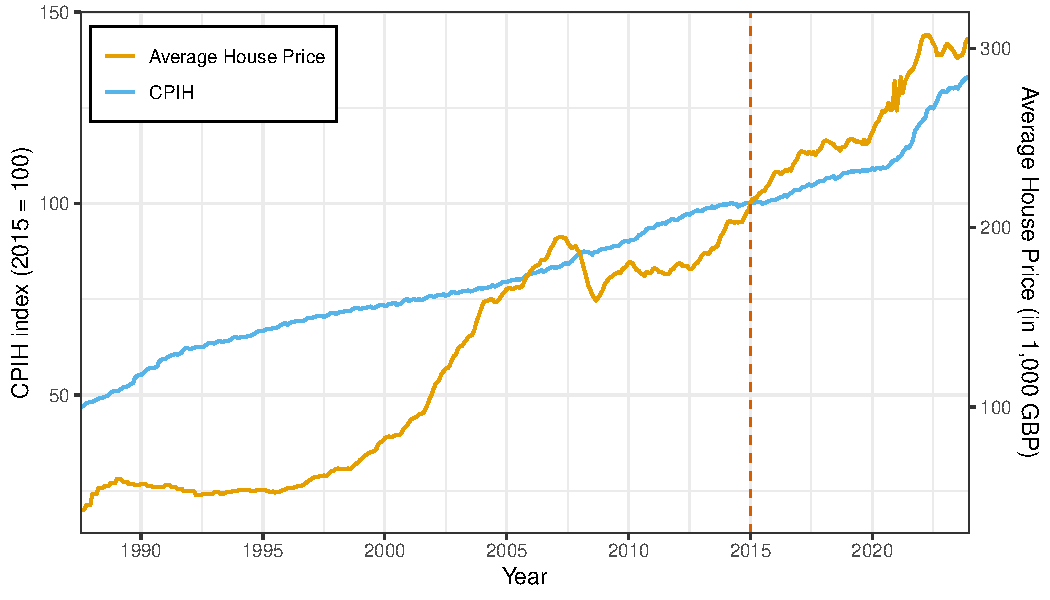
\includegraphics[width=0.8\linewidth]{figure/plot_inflation-1} 

}

\caption[Increase in average house price in England versus increase in inflation (CPIH)]{Increase in average house price in England versus increase in inflation (CPIH).}\label{fig:plot_inflation}
\end{figure}

\end{knitrout}

In Figure \ref{fig:plot_inflation}, we observe that the average house price series clearly increased faster than inflation since 2015. More specifically, the house price series increased by 43.3\% since 2015, while the CPIH index increased by 32.9\%. Also since 1988-01-01 (i.e., the first date for which both inflation and price data are available) the house price in England increased faster than inflation, with a value of 616\% and 183.4\%, respectively. 




\item Finally, we investigate whether seasonal patterns are present in the average house price changes of the United Kingdom. We do this by plotting the month-over-month percentage changes in average house prices, where the observations are grouped by month and coloured by decade in a beeswarm plot. The resulting plot is given in Figure \ref{fig:plot_beeswarm}. The large black dots in the figure, which correspond to the mean value, indicate that the average monthly change in UK house price is larger in the spring/summer period than in the autumn/winter period. This observation could potentially be explained by the weather. For instance, in the winter period it gets dark early, which might reduce the number of visits by potential buyers. Moreover, Figure \ref{fig:plot_beeswarm} annotates the observation associated with the largest monthly price drop in the UK. We observe that this drop happened in July 2021, when the average house price declined by 4.7\% in a single month. Interestingly, July 2021 is also associated with record-breaking temperatures in the UK, and there were COVID-19 restrictions in place. These events might explain the large drop in average house price. 

\begin{knitrout}
\definecolor{shadecolor}{rgb}{0.969, 0.969, 0.969}\color{fgcolor}\begin{figure}[H]

{\centering 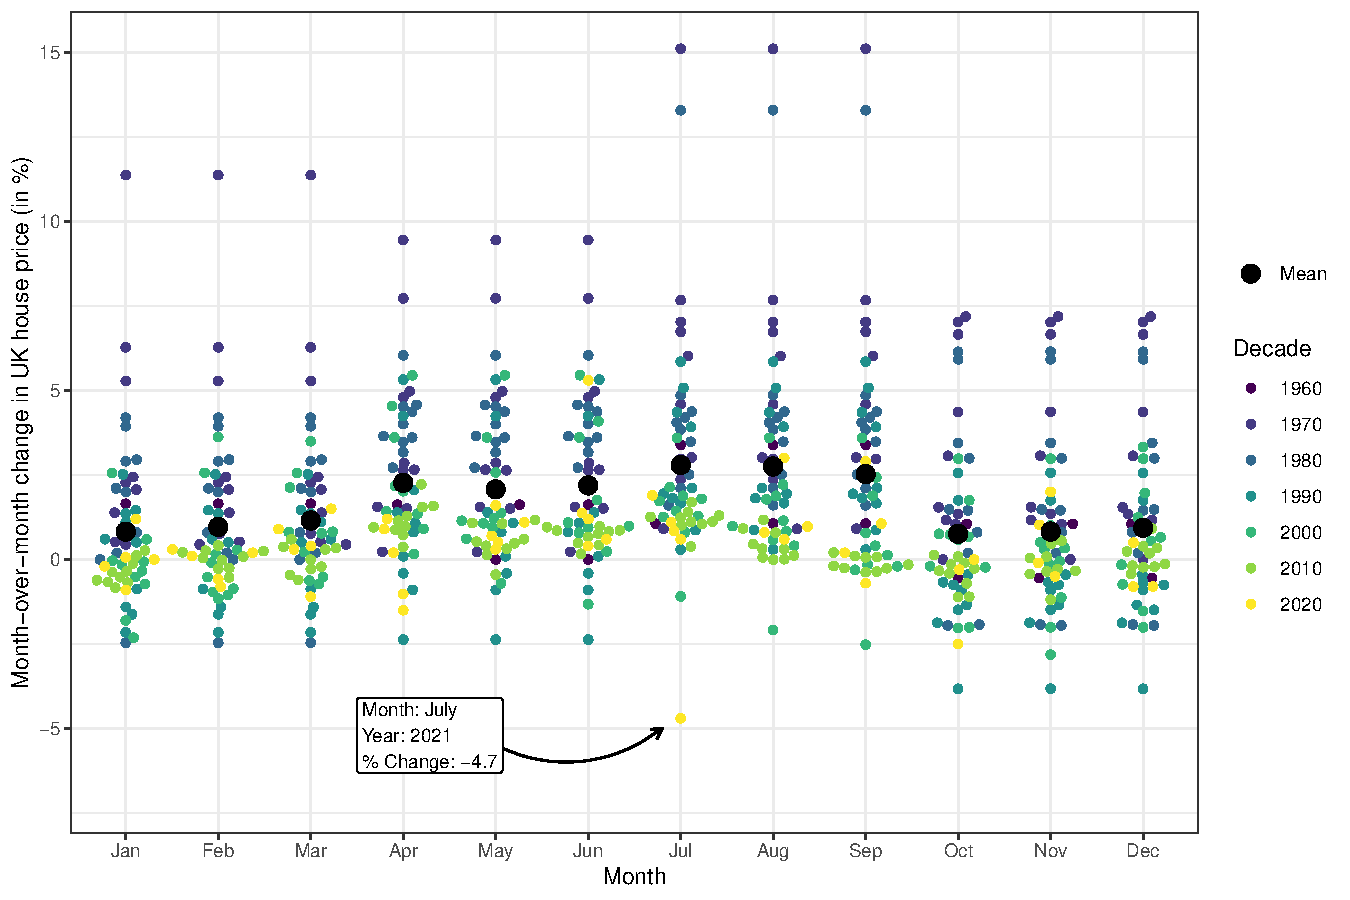
\includegraphics[width=1\linewidth]{figure/plot_beeswarm-1} 

}

\caption[Beeswarm plot for the month-over-month percentage change in average house prices in the UK]{Beeswarm plot for the month-over-month percentage change in average house prices in the UK}\label{fig:plot_beeswarm}
\end{figure}

\end{knitrout}




\end{enumerate}






\section{Chemical similarity}

\begin{enumerate}



\item In this section, we analyse the amino-acid data in the CSV file \code{AA-NNAA-FP.csv}. First, we load the dataset into R. 

\begin{knitrout}
\definecolor{shadecolor}{rgb}{0.969, 0.969, 0.969}\color{fgcolor}\begin{kframe}
\begin{alltt}
\hldef{amino_acids} \hlkwb{<-} \hlkwd{read_csv}\hldef{(}\hlsng{"AA-NNAA-FP.csv"}\hldef{,} \hlkwc{progress} \hldef{=} \hlnum{FALSE}\hldef{)}
\end{alltt}
\end{kframe}
\end{knitrout}

The resulting dataframe has 2994 rows (i.e., amino acids) and 7 columns. We obtain the column names with by running the following expression in R:

\begin{knitrout}
\definecolor{shadecolor}{rgb}{0.969, 0.969, 0.969}\color{fgcolor}\begin{kframe}
\begin{alltt}
\hldef{amino_acids} \hlopt
  \hlkwd{colnames}\hldef{()} \hlopt
  \hlkwd{kable}\hldef{(}\hlkwc{col.names} \hldef{=} \hlkwd{c}\hldef{(}\hlsng{"Column Names"}\hldef{))}
\end{alltt}
\end{kframe}
\begin{tabular}{l}
\hline
Column Names\\
\hline
Name\\
\hline
IsNatural\\
\hline
SMILES\\
\hline
TotalCharge\\
\hline
clogP\\
\hline
xlogP\\
\hline
FP\\
\hline
\end{tabular}

\end{knitrout}

Next, we would like to know the number of natural and non-natural amino acids in our sample. For this purpose, we use the \code{isNatural} column, which equals 1 when the amino acid is natural and 0 otherwise. 

\begin{knitrout}
\definecolor{shadecolor}{rgb}{0.969, 0.969, 0.969}\color{fgcolor}\begin{kframe}
\begin{alltt}
\hldef{amino_acids} \hlopt
  \hlkwd{group_by}\hldef{(IsNatural)} \hlopt
  \hlkwd{summarize}\hldef{(}\hlkwc{Count} \hldef{=} \hlkwd{n}\hldef{())} \hlopt
  \hlkwd{kable}\hldef{()}
\end{alltt}
\end{kframe}
\begin{tabular}{r|r}
\hline
IsNatural & Count\\
\hline
0 & 2950\\
\hline
1 & 44\\
\hline
\end{tabular}

\end{knitrout}

In the table above, we observe that our dataset contains 44 natural amino acids and 2950 non-natural amino acids. Note that our dataset contains more than 20 natural amino acids, which might seem like a mistake. However, our dataset also contains the natural amino acids of the \textit{zwitterionic} form. When we take this into account, we observe that our dataset contains 19 \textit{non-zwitterionic} natural amino acids, as can be seen in the table below. 

\begin{knitrout}
\definecolor{shadecolor}{rgb}{0.969, 0.969, 0.969}\color{fgcolor}\begin{kframe}
\begin{alltt}
\hldef{amino_acids} \hlopt
  \hlkwd{mutate}\hldef{(}
    \hlkwc{IsZwitterionic} \hldef{=} \hlkwd{as.integer}\hldef{(}\hlkwd{str_detect}\hldef{(Name,} \hlkwc{pattern} \hldef{=} \hlsng{"Zwitterionic"}\hldef{))}
  \hldef{)} \hlopt
  \hlkwd{group_by}\hldef{(IsNatural, IsZwitterionic)} \hlopt
  \hlkwd{summarize}\hldef{(}\hlkwc{Count} \hldef{=} \hlkwd{n}\hldef{())} \hlopt
  \hlkwd{kable}\hldef{()}
\end{alltt}
\end{kframe}
\begin{tabular}{r|r|r}
\hline
IsNatural & IsZwitterionic & Count\\
\hline
0 & 0 & 2950\\
\hline
1 & 0 & 19\\
\hline
1 & 1 & 25\\
\hline
\end{tabular}

\end{knitrout}




\item Next, we separate the dataframe \code{amino\_acids} into two new dataframes, \code{dfAA} and \code{dfNNAA}. \code{dfAA} contains the natural amino acids (AAs). Similarly, \code{dfNNAA} contains the non-natural amino acids (NNAAs). 

\begin{knitrout}
\definecolor{shadecolor}{rgb}{0.969, 0.969, 0.969}\color{fgcolor}\begin{kframe}
\begin{alltt}
\hldef{dfAA} \hlkwb{<-} \hldef{amino_acids} \hlopt
  \hlkwd{filter}\hldef{(IsNatural} \hlopt{==} \hlnum{1}\hldef{)}
\hldef{dfNNAA} \hlkwb{<-} \hldef{amino_acids} \hlopt
  \hlkwd{filter}\hldef{(IsNatural} \hlopt{==} \hlnum{0}\hldef{)}
\end{alltt}
\end{kframe}
\end{knitrout}

The last column in these dataframes is \code{FP}, which contains the ECFP4 2048-bit fingerprints. We would like to test whether all these fingerprints are indeed 2048 bits long. We check this with the expression given below. Note that the fingerprints are stored as strings in \code{amino\_acids}, where the bits are separated by spaces. 

\begin{knitrout}
\definecolor{shadecolor}{rgb}{0.969, 0.969, 0.969}\color{fgcolor}\begin{kframe}
\begin{alltt}
\hlkwd{test_that}\hldef{(}\hlsng{"All fingerprints in dataframe are 2048 bits long"}\hldef{, \{}
  \hlkwd{expect_true}\hldef{(}
    \hlkwd{all}\hldef{(}
      \hldef{amino_acids} \hlopt
        \hlkwd{pull}\hldef{(FP)} \hlopt
        \hlkwd{str_split}\hldef{(}\hlkwc{pattern} \hldef{=} \hlsng{" "}\hldef{)} \hlopt
        \hlkwd{sapply}\hldef{(}\hlkwc{FUN} \hldef{= length)}
      \hlopt{==} \hlnum{2048}
    \hldef{)}
  \hldef{)}
\hldef{\})}
\end{alltt}
\begin{verbatim}
## Test passed
\end{verbatim}
\end{kframe}
\end{knitrout}

Since the test is passed, we conclude that all the fingerprints in the original dataframe are indeed 2048 bits long. 




\item Now that we know all fingerprints are of the correct length, it is time to develop our first function to calculate the Tanimoto similarity measure. This function, which is named \code{get\_tanimoto\_similarity}, calculates the Tanimoto similarity measure for two fingerprints by comparing each pair of bits using a for loop. The function is defined as follows. 

\begin{knitrout}
\definecolor{shadecolor}{rgb}{0.969, 0.969, 0.969}\color{fgcolor}\begin{kframe}
\begin{alltt}
\hldef{get_tanimoto_similarity} \hlkwb{<-} \hlkwa{function}\hldef{(}\hlkwc{fp1}\hldef{,} \hlkwc{fp2}\hldef{) \{}
  \hldef{n_intersection} \hlkwb{<-} \hlnum{0}
  \hldef{n_union} \hlkwb{<-} \hlnum{0}

  \hlkwa{for} \hldef{(i} \hlkwa{in} \hlkwd{seq_along}\hldef{(fp1)) \{}
    \hlkwa{if} \hldef{(fp1[i]} \hlopt{||} \hldef{fp2[i]) \{}
      \hldef{n_union} \hlkwb{<-} \hldef{n_union} \hlopt{+} \hlnum{1}
      \hlkwa{if} \hldef{(fp1[i]} \hlopt{&&} \hldef{fp2[i]) \{}
        \hldef{n_intersection} \hlkwb{<-} \hldef{n_intersection} \hlopt{+} \hlnum{1}
      \hldef{\}}
    \hldef{\}}
  \hldef{\}}

  \hlkwa{if} \hldef{(n_union} \hlopt{==} \hlnum{0}\hldef{) \{}
    \hlkwd{return}\hldef{(}\hlnum{1.0}\hldef{)}
  \hldef{\}}
  \hldef{n_intersection} \hlopt{/} \hldef{n_union}
\hldef{\}}
\end{alltt}
\end{kframe}
\end{knitrout}

In order to prevent a division by zero, we include a if-condition before we calculate the Tanimoto similarity measure and return the output. The only situation that can result in a division by zero is when both fingerprints contain only zeroes. This means that no single chemical substructure is present in any of the two fingerprints. Even though this situation is very unlikely to occur, and might rather be an indicator of a typo in the data, we do take it explicitly into account here. Formally, two fingerprints with only zeroes are identical and, thus, the Tanimoto similarity measure should be one. \par

Furthermore, in the function above we assume that the fingerprints provided as arguments (\code{fp1} and \code{fp2}) are integer vectors of binary numbers. However, as we mentioned before, the fingerprints in the original dataframe are strings. We decide to convert the strings to integer vectors outside the function above (and any function below), since this is more efficient (but it is maybe less beneficial when someone cares about storage). For example, if we would like to compare all the fingerprints to all other fingerprints, the number of conversions from string to integer vector would be way less when we do this outside the function call (only once) than when we do this inside the function. \par 

The tests below check that the numeric value returned by \code{get\_tanimoto\_similarity} is never negative or greater than 1.

\begin{knitrout}
\definecolor{shadecolor}{rgb}{0.969, 0.969, 0.969}\color{fgcolor}\begin{kframe}
\begin{alltt}
\hlkwd{test_that}\hldef{(}\hlsng{"Identical fingerprints give tanimoto similarity of 1"}\hldef{, \{}
  \hldef{fp1} \hlkwb{<-} \hlkwd{c}\hldef{(}\hlnum{1}\hldef{,} \hlnum{0}\hldef{,} \hlnum{1}\hldef{,} \hlnum{0}\hldef{,} \hlnum{1}\hldef{)}
  \hldef{fp2} \hlkwb{<-} \hldef{fp1}
  \hlkwd{expect_equal}\hldef{(}
    \hlkwd{get_tanimoto_similarity}\hldef{(fp1, fp2),}
    \hlnum{1}
  \hldef{)}
\hldef{\})}
\end{alltt}
\begin{verbatim}
## Test passed
\end{verbatim}
\begin{alltt}
\hlkwd{test_that}\hldef{(}\hlsng{"Completely different fingerprints have similarity of 0"}\hldef{, \{}
  \hldef{fp1} \hlkwb{<-} \hlkwd{c}\hldef{(}\hlnum{1}\hldef{,} \hlnum{0}\hldef{,} \hlnum{1}\hldef{,} \hlnum{0}\hldef{,} \hlnum{1}\hldef{)}
  \hldef{fp2} \hlkwb{<-} \hlkwd{c}\hldef{(}\hlnum{0}\hldef{,} \hlnum{1}\hldef{,} \hlnum{0}\hldef{,} \hlnum{1}\hldef{,} \hlnum{0}\hldef{)}
  \hlkwd{expect_equal}\hldef{(}
    \hlkwd{get_tanimoto_similarity}\hldef{(fp1, fp2),}
    \hlnum{0}
  \hldef{)}
\hldef{\})}
\end{alltt}
\begin{verbatim}
## Test passed
\end{verbatim}
\begin{alltt}
\hlkwd{test_that}\hldef{(}\hlsng{"Two fingerprints have similarity between 0 and 1"}\hldef{, \{}
  \hldef{fp1} \hlkwb{<-} \hlkwd{c}\hldef{(}\hlnum{1}\hldef{,} \hlnum{0}\hldef{,} \hlnum{1}\hldef{,} \hlnum{0}\hldef{,} \hlnum{1}\hldef{)}
  \hldef{fp2} \hlkwb{<-} \hlkwd{c}\hldef{(}\hlnum{0}\hldef{,} \hlnum{0}\hldef{,} \hlnum{1}\hldef{,} \hlnum{1}\hldef{,} \hlnum{1}\hldef{)}
  \hldef{value} \hlkwb{<-} \hlkwd{get_tanimoto_similarity}\hldef{(fp1, fp2)}
  \hlkwd{expect_true}\hldef{(value} \hlopt{<=} \hlnum{1} \hlopt{&} \hldef{value} \hlopt{>=} \hlnum{0}\hldef{)}
\hldef{\})}
\end{alltt}
\begin{verbatim}
## Test passed
\end{verbatim}
\begin{alltt}
\hlkwd{test_that}\hldef{(}\hlsng{"Two fingerprints with only zeroes have similarity of 1"}\hldef{, \{}
  \hldef{fp1} \hlkwb{<-} \hlkwd{rep}\hldef{(}\hlnum{0}\hldef{,} \hlkwc{times} \hldef{=} \hlnum{5}\hldef{)}
  \hldef{fp2} \hlkwb{<-} \hlkwd{rep}\hldef{(}\hlnum{0}\hldef{,} \hlkwc{times} \hldef{=} \hlnum{5}\hldef{)}
  \hlkwd{expect_equal}\hldef{(}
    \hlkwd{get_tanimoto_similarity}\hldef{(fp1, fp2),}
    \hlnum{1}
  \hldef{)}
\hldef{\})}
\end{alltt}
\begin{verbatim}
## Test passed
\end{verbatim}
\end{kframe}
\end{knitrout}




\item Instead of using a for-loop it is probably more efficient to implement the Tanimoto similarity calculation using vectorized R. This function, named \code{get\_tanimoto\_vectorized}, is defined as follows:

\begin{knitrout}
\definecolor{shadecolor}{rgb}{0.969, 0.969, 0.969}\color{fgcolor}\begin{kframe}
\begin{alltt}
\hldef{get_tanimoto_vectorized} \hlkwb{<-} \hlkwa{function}\hldef{(}\hlkwc{fp1}\hldef{,} \hlkwc{fp2}\hldef{) \{}
  \hldef{n_union} \hlkwb{<-} \hlkwd{sum}\hldef{(fp1} \hlopt{|} \hldef{fp2)}
  \hldef{n_intersection} \hlkwb{<-} \hlkwd{sum}\hldef{(fp1} \hlopt{&} \hldef{fp2)}

  \hlkwa{if} \hldef{(n_union} \hlopt{==} \hlnum{0}\hldef{) \{}
    \hlkwd{return}\hldef{(}\hlnum{1.0}\hldef{)}
  \hldef{\}}
  \hldef{n_intersection} \hlopt{/} \hldef{n_union}
\hldef{\}}
\end{alltt}
\end{kframe}
\end{knitrout}




\item For our third implementation of the Tanimoto simularity calculation, we use the \code{bitops} package. It provides functions to perform bitwise comparisons of integer vectors. Using these function, we define the following \code{get\_tanimoto\_bitops} function.  

\begin{knitrout}
\definecolor{shadecolor}{rgb}{0.969, 0.969, 0.969}\color{fgcolor}\begin{kframe}
\begin{alltt}
\hldef{get_tanimoto_bitops} \hlkwb{<-} \hlkwa{function}\hldef{(}\hlkwc{fp1}\hldef{,} \hlkwc{fp2}\hldef{) \{}
  \hldef{n_union} \hlkwb{<-} \hlkwd{sum}\hldef{(bitops}\hlopt{::}\hlkwd{bitOr}\hldef{(fp1, fp2))}
  \hldef{n_intersection} \hlkwb{<-} \hlkwd{sum}\hldef{(bitops}\hlopt{::}\hlkwd{bitAnd}\hldef{(fp1, fp2))}

  \hlkwa{if} \hldef{(n_union} \hlopt{==} \hlnum{0}\hldef{) \{}
    \hlkwd{return}\hldef{(}\hlnum{1.0}\hldef{)}
  \hldef{\}}
  \hldef{n_intersection} \hlopt{/} \hldef{n_union}
\hldef{\}}
\end{alltt}
\end{kframe}
\end{knitrout}




\item Finally, we define the C++ function \code{get\_tanimoto\_Rcpp} in R using the \code{Rcpp} package. 

\begin{knitrout}
\definecolor{shadecolor}{rgb}{0.969, 0.969, 0.969}\color{fgcolor}\begin{kframe}
\begin{alltt}
\hldef{Rcpp}\hlopt{::}\hlkwd{cppFunction}\hldef{(}\hlsng{"
double get_tanimoto_Rcpp(IntegerVector fp1, IntegerVector fp2) \{
    double n_intersection = 0; 
    double n_union = 0; 
    
    for (int i = 0; i < fp1.size(); i++) \{
        if (fp1[i] == 1 || fp2[i] == 1) \{
            n_union++;
            if (fp1[i] == 1 && fp2[i] == 1) \{
                n_intersection++;
            \}
        \}
    \}
    
    if (n_union == 0) \{
        return 1.0; 
    \}
    return n_intersection / n_union; 
\}                 
"}\hldef{)}
\end{alltt}
\end{kframe}
\end{knitrout}




\item It is important to test that all the functions that we defined above give the same Tanimoto similarity measure. Therefore, we use the \code{testthat} package to define an unit test for the equality of output. This test is given below, and uses the first natural amino acid in \code{dfAA} and non-natural amino acid in \code{dfNNAA} as input arguments. 

\begin{knitrout}
\definecolor{shadecolor}{rgb}{0.969, 0.969, 0.969}\color{fgcolor}\begin{kframe}
\begin{alltt}
\hlkwd{test_that}\hldef{(}\hlsng{"All functions generate the same Tanimoto similarity result"}\hldef{, \{}
  \hldef{fp1} \hlkwb{<-} \hlkwd{as.integer}\hldef{(}\hlkwd{str_split_1}\hldef{(dfAA}\hlopt{$}\hldef{FP[}\hlnum{1}\hldef{],} \hlkwc{pattern} \hldef{=} \hlsng{" "}\hldef{))}
  \hldef{fp2} \hlkwb{<-} \hlkwd{as.integer}\hldef{(}\hlkwd{str_split_1}\hldef{(dfNNAA}\hlopt{$}\hldef{FP[}\hlnum{1}\hldef{],} \hlkwc{pattern} \hldef{=} \hlsng{" "}\hldef{))}
  \hlkwd{expect_equal}\hldef{(}
    \hlkwd{get_tanimoto_similarity}\hldef{(fp1, fp2),}
    \hlkwd{get_tanimoto_vectorized}\hldef{(fp1, fp2)}
  \hldef{)}
  \hlkwd{expect_equal}\hldef{(}
    \hlkwd{get_tanimoto_vectorized}\hldef{(fp1, fp2),}
    \hlkwd{get_tanimoto_bitops}\hldef{(fp1, fp2)}
  \hldef{)}
  \hlkwd{expect_equal}\hldef{(}
    \hlkwd{get_tanimoto_bitops}\hldef{(fp1, fp2),}
    \hlkwd{get_tanimoto_Rcpp}\hldef{(fp1, fp2)}
  \hldef{)}
\hldef{\})}
\end{alltt}
\begin{verbatim}
## Test passed
\end{verbatim}
\end{kframe}
\end{knitrout}




\item Ultimately, we want to know which implementation calculates the Tanimoto similarity the fastest. For this reason, we will benchmark the four implementations below. We define the function \code{get\_running\_times}, which gives the running times in seconds (by default, \code{unit} = ``s") for each Tanimoto function that is runned \code{runs} times. 

\begin{knitrout}
\definecolor{shadecolor}{rgb}{0.969, 0.969, 0.969}\color{fgcolor}\begin{kframe}
\begin{alltt}
\hldef{get_running_times} \hlkwb{<-} \hlkwa{function}\hldef{(}\hlkwc{runs}\hldef{,} \hlkwc{unit} \hldef{=} \hlsng{"s"}\hldef{) \{}
  \hldef{fp1} \hlkwb{<-} \hlkwd{as.integer}\hldef{(}\hlkwd{str_split_1}\hldef{(dfAA}\hlopt{$}\hldef{FP[}\hlnum{1}\hldef{],} \hlkwc{pattern} \hldef{=} \hlsng{" "}\hldef{))}
  \hldef{fp2} \hlkwb{<-} \hlkwd{as.integer}\hldef{(}\hlkwd{str_split_1}\hldef{(dfNNAA}\hlopt{$}\hldef{FP[}\hlnum{1}\hldef{],} \hlkwc{pattern} \hldef{=} \hlsng{" "}\hldef{))}
  \hldef{times} \hlkwb{<-} \hlkwd{microbenchmark}\hldef{(}
    \hlsng{"R loop"} \hldef{=} \hlkwd{get_tanimoto_similarity}\hldef{(fp1, fp2),}
    \hlsng{"R vectorized"} \hldef{=} \hlkwd{get_tanimoto_vectorized}\hldef{(fp1, fp2),}
    \hlkwc{bitops} \hldef{=} \hlkwd{get_tanimoto_bitops}\hldef{(fp1, fp2),}
    \hlkwc{Rcpp} \hldef{=} \hlkwd{get_tanimoto_Rcpp}\hldef{(fp1, fp2),}
    \hlkwc{times} \hldef{= runs,}
    \hlkwc{unit} \hldef{= unit}
  \hldef{)}
  \hlkwd{summary}\hldef{(times)[,} \hlkwd{c}\hldef{(}\hlsng{"expr"}\hldef{,} \hlsng{"mean"}\hldef{,} \hlsng{"neval"}\hldef{)]}
\hldef{\}}
\end{alltt}
\end{kframe}
\end{knitrout}


\begin{enumerate}

\item First, we use \code{get\_running\_times} to obtain the running times (in seconds) of the four Tanimoto implementations, and for different number of \code{runs}. More specifically, we consider the running times when each implementation is called 1000, 5000, 10000, 25000, 50000, 75000, or 100000 times. The running times are given in Table \ref{tab:table_running_times}. 

\begin{knitrout}
\definecolor{shadecolor}{rgb}{0.969, 0.969, 0.969}\color{fgcolor}\begin{kframe}
\begin{alltt}
\hldef{seq_runs} \hlkwb{<-} \hlkwd{c}\hldef{(}\hlnum{1}\hldef{,} \hlnum{5}\hldef{,} \hlnum{10}\hldef{,} \hlnum{25}\hldef{,} \hlnum{50}\hldef{,} \hlnum{75}\hldef{,} \hlnum{100}\hldef{)} \hlopt{*} \hlnum{1000}

\hldef{total_run_times} \hlkwb{<-} \hlkwd{bind_rows}\hldef{(}
  \hlkwd{lapply}\hldef{(seq_runs,} \hlkwc{FUN} \hldef{=} \hlkwa{function}\hldef{(}\hlkwc{x}\hldef{)} \hlkwd{get_running_times}\hldef{(}\hlkwc{runs} \hldef{= x))}
\hldef{)} \hlopt
  \hlkwd{mutate}\hldef{(}\hlkwc{total} \hldef{= mean} \hlopt{*} \hldef{neval)} \hlopt
  \hlkwd{select}\hldef{(}\hlopt{-}\hldef{mean)}

\hldef{total_run_times} \hlopt
  \hlkwd{pivot_wider}\hldef{(}\hlkwc{names_from} \hldef{= expr,} \hlkwc{values_from} \hldef{= total)} \hlopt
  \hlkwd{rename}\hldef{(}\hlkwc{Runs} \hldef{= neval)} \hlopt
  \hlkwd{kbl}\hldef{(}
    \hlkwc{digits} \hldef{=} \hlnum{2}\hldef{,}
    \hlkwc{caption} \hldef{=} \hlkwd{paste0}\hldef{(}\hlsng{"Running times (in seconds) for the four "}\hldef{,}
                     \hlsng{"Tanimoto similarity functions defined in "}\hldef{,}
                     \hlsng{"this paper."}\hldef{),}
    \hlkwc{booktabs} \hldef{=} \hlnum{TRUE}\hldef{,}
    \hlkwc{linesep} \hldef{=} \hlsng{""}\hldef{,}
    \hlkwc{table.envir} \hldef{=} \hlsng{"table\} \textbackslash{}\textbackslash{}captionsetup\{margin = 20pt"}
  \hldef{)} \hlopt
  \hlkwd{column_spec}\hldef{(}\hlnum{1}\hlopt{:}\hlnum{5}\hldef{,} \hlkwc{width} \hldef{=} \hlsng{"2.5 cm"}\hldef{)} \hlopt
  \hlkwd{kable_paper}\hldef{(}\hlkwc{latex_options} \hldef{=} \hlkwd{c}\hldef{(}\hlsng{"HOLD_position"}\hldef{))}
\end{alltt}
\end{kframe}\begin{table}[H] \captionsetup{margin = 20pt}
\centering
\caption{\label{tab:table_running_times}Running times (in seconds) for the four Tanimoto similarity functions defined in this paper.}
\centering
\begin{tabular}[t]{>{\raggedleft\arraybackslash}p{2.5 cm}>{\raggedleft\arraybackslash}p{2.5 cm}>{\raggedleft\arraybackslash}p{2.5 cm}>{\raggedleft\arraybackslash}p{2.5 cm}>{\raggedleft\arraybackslash}p{2.5 cm}}
\toprule
Runs & R loop & R vectorized & bitops & Rcpp\\
\midrule
1000 & 0.13 & 0.02 & 0.04 & 0.01\\
5000 & 0.61 & 0.08 & 0.22 & 0.03\\
10000 & 1.29 & 0.17 & 0.42 & 0.05\\
25000 & 3.10 & 0.43 & 1.09 & 0.14\\
50000 & 6.32 & 0.86 & 2.16 & 0.28\\
75000 & 9.42 & 1.33 & 3.27 & 0.41\\
100000 & 12.21 & 1.95 & 4.61 & 0.55\\
\bottomrule
\end{tabular}
\end{table} \captionsetup{margin = 20pt}

\end{knitrout}

We observe that the C++ implementation, with the function \code{get\_tanimoto\_Rcpp}, has the lowest running times. Furthermore, the remaining implementations can be ordered from low to high running times by: ``R vectorized", ``bitops" and ``R loop". 




\item Next, we plot the running times for each method against the number of repetitions. We use the following R code to generate the figure. 

\begin{knitrout}
\definecolor{shadecolor}{rgb}{0.969, 0.969, 0.969}\color{fgcolor}\begin{kframe}
\begin{alltt}
\hlkwd{ggplot}\hldef{(}
  \hlkwc{data} \hldef{= total_run_times,}
  \hlkwc{mapping} \hldef{=} \hlkwd{aes}\hldef{(}
    \hlkwc{x} \hldef{= neval,}
    \hlkwc{y} \hldef{= total,}
    \hlkwc{linetype} \hldef{= expr,}
    \hlkwc{colour} \hldef{= expr}
  \hldef{)}
\hldef{)} \hlopt{+}
  \hlkwd{geom_line}\hldef{(}\hlkwc{linewidth} \hldef{=} \hlnum{0.7}\hldef{)} \hlopt{+}
  \hlkwd{scale_colour_manual}\hldef{(}\hlkwc{values} \hldef{= cbPalette[}\hlopt{-}\hlnum{1}\hldef{])} \hlopt{+}
  \hlkwd{scale_x_continuous}\hldef{(}\hlkwc{breaks} \hldef{= seq_runs,} \hlkwc{minor_breaks} \hldef{=} \hlkwa{NULL}\hldef{)} \hlopt{+}
  \hlkwd{labs}\hldef{(}
    \hlkwc{x} \hldef{=} \hlsng{"Number of Repetitions"}\hldef{,}
    \hlkwc{y} \hldef{=} \hlsng{"Time (seconds)"}\hldef{,}
    \hlkwc{linetype} \hldef{=} \hlsng{"Method"}\hldef{,}
    \hlkwc{colour} \hldef{=} \hlsng{"Method"}\hldef{,}
    \hlkwc{title} \hldef{=} \hlsng{"Performance Comparison of Tanimoto Similarity Methods"}
  \hldef{)} \hlopt{+}
  \hlkwd{theme}\hldef{(}
    \hlkwc{legend.position} \hldef{=} \hlkwd{c}\hldef{(}\hlnum{0.08}\hldef{,} \hlnum{0.82}\hldef{),}
    \hlkwc{legend.background} \hldef{=} \hlkwd{element_rect}\hldef{(}\hlkwc{colour} \hldef{=} \hlsng{"black"}\hldef{)}
  \hldef{)}
\end{alltt}
\end{kframe}

{\centering 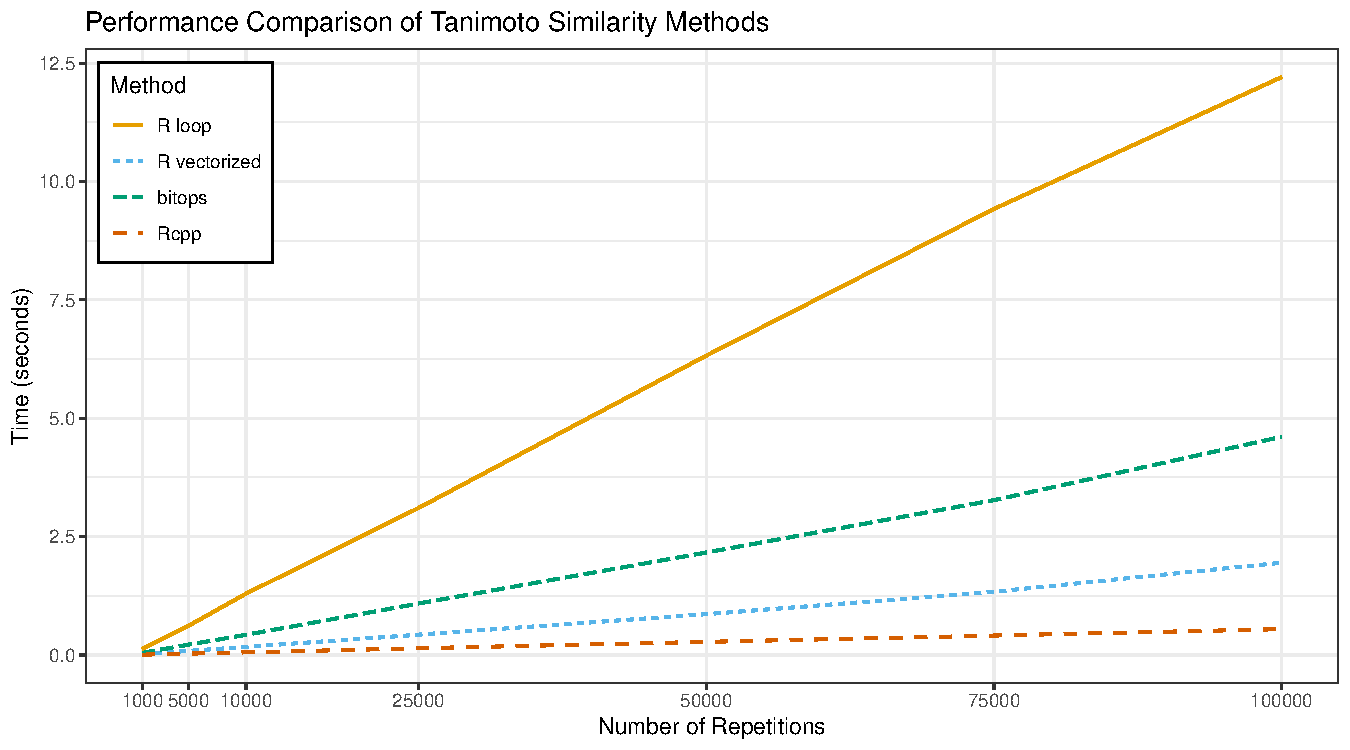
\includegraphics[width=\maxwidth]{figure/plot_running_times-1} 

}


\end{knitrout}

In the figure above, we observe that, for each method, the running time increases linearly with the number of repetitions. However, the slope of this linear relationship differs between the methods. Especially, the running time for the ``R loop" method (\code{get\_tanimoto\_similarity}) increases faster than the running time for other methods. Furthermore, it is not surprising that we observe a linear relationship because the size of the input arguments stays the same (i.e., each fingerprints has 2048 bits). Additionally, since no randomness is involved in the calculation of the Tanimoto similarity, the average running time is likely constant for these large number or repetitions. Thus, the total running time will increase by a constant factor for each additional repetition.




\item Now, we will analyse the time-complexity of the four Tanimoto algorithms using the Big-O notation. The figure above might suggest that the time-complexity is linear for each method. However, note that this figure does not show how the running time increases as a function of the size of the input arguments (i.e., the number of bits in each fingerprint). Instead, the complexity of an algorithm is related to this relationship between input size and number of operations (which can be related to running time if we assume that each operation takes a fixed amount of time). Let $N$ be the length of the fingerprint-vectors (i.e., the number of bits). Then, the Big-O notation for each implementation can be derived as follows: 

\textbf{R loop}
\begin{enumerate}
\item We loop over the length of the fingerprints ($N$). Thus, the number of operations we perform inside this loop should be multiplied by a factor $N$. 

\item In each iteration, we compare the two bits at the corresponding positions in \code{fp1} and \code{fp2} (i.e., the two fingerprints). Then, given this comparison, we perform a fixed number of operations (i.e., does not increase with the size of any input arguments). Thus, the complexity for each iteration is $\mathcal{O}(1)$. 

\item After running the loop, we check the value of one variable, which can be seen as one operation. Then, we immediately return the desired result. 

\item \textbf{Conclusion:} the complexity is roughly given by $\mathcal{O}(N) * \mathcal{O}(1) + \mathcal{O}(1)$, which is equivalent to $\mathcal{O}(N)$. 
\end{enumerate}


\textbf{R vectorized}
\begin{enumerate}
\item First, we use the element-wise OR and AND operators on the two fingerprints of length $N$. So, these operations have a time-complexity of $\mathcal{O}(2N) = \mathcal{O}(N)$. We are left with two boolean vectors of length $N$. 

\item Then, we sum over the two boolean vectors to obtain two numeric values (\code{n\_union} and \code{n\_intersection}). These operations again have a complexity of roughly $\mathcal{O}(2N) = \mathcal{O}(N)$.

\item Finally, we again check one variable to avoid a division by zero, which gives one additional operation. After that, we return the final result. 

\item \textbf{Conclusion:} the complexity is roughly $\mathcal{O}(N) + \mathcal{O}(N) + \mathcal{O}(1)$, which can be summarized as $\mathcal{O}(N)$. Given the first 2 steps above, you might believe that the complexity is given by $\mathcal{O}(N * N)$. However, note that the sum is performed after we compared all the $N$ pairs of bits. We do not sum over $N$ elements for each pair of bits we compare, which would give $\mathcal{O}(N^2)$. 
\end{enumerate}


\textbf{Bitops} \newline
The same analysis as for ``R vectorized". However, we use the \code{bitAnd} and \code{bitOr} functions instead of the element-wise ``\&" and ``$|$" equivalents. We assume that the complexity of both functions is $\mathcal{O}(N)$. Then, the complexity of \code{get\_tanimoto\_bitops} is also $\mathcal{O}(N)$. 

\textbf{Rcpp} \newline
The C++ function is exactly the same as the \code{get\_tanimoto\_similarity} function. The only difference is that it is implemented in C++ instead of R. Therefore, the same analysis as for ``R loop" holds here. Thus, the complexity of \code{get\_tanimoto\_Rcpp} is $\mathcal{O}(N)$.  




\item All in all, we observe that the C++ implementation has the lowest running times. Given the analysis above, this cannot be explained by the time-complexity of the algorithms, since all implementations have the same complexity. Instead C++ is just faster. For instance, in the lecture notes it is written that C++ runs for-loops faster. This could potentially explain why \code{get\_tanimoto\_Rcpp} is faster than the other functions. 

\end{enumerate}




\item In this section, we will make three tables that show the most, second most, and third most similar non-natural amino acids (NNAAs) for each natural amino acid (AA). The final tables report the natural AAs in alphabetical order. We use our \code{get\_tanimoto\_Rcpp} function (i.e., our fastest function) to calculate the Tanimoto similarities between all NNAAs in \code{dfNNAA} and AAs in \code{dfAA}. In order to calculate these similarity measures, we need the fingerprints as integer vectors. As we argued earlier, we prefer to convert all fingerprint strings to integer vectors only once. We store all the bit-vectors in lists by running the following R expression:

\begin{knitrout}
\definecolor{shadecolor}{rgb}{0.969, 0.969, 0.969}\color{fgcolor}\begin{kframe}
\begin{alltt}
\hldef{AA_FP_list} \hlkwb{<-} \hlkwd{lapply}\hldef{(}
  \hlkwc{X} \hldef{=} \hlkwd{str_split}\hldef{(dfAA}\hlopt{$}\hldef{FP,} \hlkwc{pattern} \hldef{=} \hlsng{" "}\hldef{),}
  \hlkwc{FUN} \hldef{= as.integer}
\hldef{)}
\hlkwd{names}\hldef{(AA_FP_list)} \hlkwb{<-} \hldef{dfAA}\hlopt{$}\hldef{Name}
\hldef{NNAA_FP_list} \hlkwb{<-} \hlkwd{lapply}\hldef{(}
  \hlkwc{X} \hldef{=} \hlkwd{str_split}\hldef{(dfNNAA}\hlopt{$}\hldef{FP,} \hlkwc{pattern} \hldef{=} \hlsng{" "}\hldef{),}
  \hlkwc{FUN} \hldef{= as.integer}
\hldef{)}
\hlkwd{names}\hldef{(NNAA_FP_list)} \hlkwb{<-} \hldef{dfNNAA}\hlopt{$}\hldef{Name}
\end{alltt}
\end{kframe}
\end{knitrout}

Then, we code a function that calculates the $n$ most similar NNAAs for each natural amino acid (AA). We use this function to make a variable \code{three\_most\_similar\_NNAAs}, which is a list and stores the \code{tibble} objects with the $n$ most similar NNAAs for each AA in \code{dfAA}. 

\begin{knitrout}
\definecolor{shadecolor}{rgb}{0.969, 0.969, 0.969}\color{fgcolor}\begin{kframe}
\begin{alltt}
\hldef{find_n_most_similar_NNAAs} \hlkwb{<-} \hlkwa{function}\hldef{(}\hlkwc{AA_FP}\hldef{,} \hlkwc{NNAA_FP_list}\hldef{,} \hlkwc{n} \hldef{=} \hlnum{3}\hldef{) \{}
  \hldef{similarity} \hlkwb{<-} \hlkwd{lapply}\hldef{(}
    \hlkwc{X} \hldef{= NNAA_FP_list,}
    \hlkwc{FUN} \hldef{=} \hlkwa{function}\hldef{(}\hlkwc{x}\hldef{)} \hlkwd{get_tanimoto_Rcpp}\hldef{(}\hlkwc{fp1} \hldef{= x,} \hlkwc{fp2} \hldef{= AA_FP)}
  \hldef{)}

  \hlkwd{tibble}\hldef{(}
    \hlkwc{NNAAName} \hldef{=} \hlkwd{names}\hldef{(similarity),}
    \hlkwc{Similarity} \hldef{=} \hlkwd{as.numeric}\hldef{(similarity)}
  \hldef{)} \hlopt
    \hlkwd{arrange}\hldef{(}\hlkwd{desc}\hldef{(Similarity))} \hlopt
    \hlkwd{head}\hldef{(}\hlkwc{n} \hldef{= n)}
\hldef{\}}

\hldef{three_most_similar_NNAAs} \hlkwb{<-} \hlkwd{lapply}\hldef{(}
  \hlkwc{X} \hldef{= AA_FP_list,}
  \hlkwc{FUN} \hldef{=} \hlkwa{function}\hldef{(}\hlkwc{x}\hldef{)} \hlkwd{find_n_most_similar_NNAAs}\hldef{(}\hlkwc{AA_FP} \hldef{= x, NNAA_FP_list)}
\hldef{)}
\end{alltt}
\end{kframe}
\end{knitrout}

Finally, we make the similarity tables with the \code{kableExtra} package. The table for a specific \code{rank} (between $1$ and $n$), and with a specific \code{caption}, is obtained by calling the function \code{make\_similarity\_table}. 

\begin{kframe}
\begin{alltt}
\hldef{make_similarity_table} \hlkwb{<-} \hlkwa{function}\hldef{(}
    \hlkwc{most_similar_NNAAs}\hldef{,}
    \hlkwc{rank}\hldef{,}
    \hlkwc{caption}\hldef{,}
    \hlkwc{label}
\hldef{) \{}
  \hlkwd{tibble}\hldef{(}
    \hlkwc{AAName} \hldef{=} \hlkwd{names}\hldef{(most_similar_NNAAs),}
    \hlkwd{bind_rows}\hldef{(}\hlkwd{lapply}\hldef{(}\hlkwc{X} \hldef{= most_similar_NNAAs,} \hlkwc{FUN} \hldef{=} \hlkwa{function}\hldef{(}\hlkwc{x}\hldef{) x[rank,]))}
  \hldef{)} \hlopt
    \hlkwd{arrange}\hldef{(AAName)} \hlopt
    \hlkwd{kbl}\hldef{(}
      \hlkwc{digits} \hldef{=} \hlnum{3}\hldef{,}
      \hlkwc{format} \hldef{=} \hlsng{"latex"}\hldef{,}
      \hlkwc{booktabs} \hldef{=} \hlnum{TRUE}\hldef{,}
      \hlkwc{caption} \hldef{= caption,}
      \hlkwc{linesep} \hldef{=} \hlsng{""}\hldef{,}
      \hlkwc{table.envir} \hldef{=} \hlsng{"table\} \textbackslash{}\textbackslash{}captionsetup\{margin = 55pt"}\hldef{,}
      \hlkwc{label} \hldef{= label}
    \hldef{)} \hlopt
    \hlkwd{kable_styling}\hldef{(}\hlkwc{latex_options} \hldef{=} \hlkwd{c}\hldef{(}\hlsng{"HOLD_position"}\hldef{),} \hlkwc{font_size} \hldef{=} \hlnum{10}\hldef{)}
\hldef{\}}

\hldef{table_input_args} \hlkwb{<-} \hlkwd{list}\hldef{(}
  \hlkwd{c}\hldef{(}\hlkwc{rank} \hldef{=} \hlnum{1}\hldef{,} \hlkwc{cap} \hldef{=} \hlsng{"Most Similar Non-natural AA"}\hldef{,} \hlkwc{lab} \hldef{=} \hlsng{"most1"}\hldef{),}
  \hlkwd{c}\hldef{(}\hlkwc{rank} \hldef{=} \hlnum{2}\hldef{,} \hlkwc{cap} \hldef{=} \hlsng{"Second Most Similar Non-natural AA"}\hldef{,} \hlkwc{lab} \hldef{=} \hlsng{"most2"}\hldef{),}
  \hlkwd{c}\hldef{(}\hlkwc{rank} \hldef{=} \hlnum{3}\hldef{,} \hlkwc{cap} \hldef{=} \hlsng{"Third Most Similar Non-natural AA"}\hldef{,} \hlkwc{lab} \hldef{=} \hlsng{"most3"}\hldef{)}
\hldef{)}
\hlkwa{for} \hldef{(args} \hlkwa{in} \hldef{table_input_args) \{}
  \hlkwd{print}\hldef{(}\hlkwd{make_similarity_table}\hldef{(}
    \hldef{three_most_similar_NNAAs,}
    \hlkwc{rank} \hldef{= args[}\hlsng{"rank"}\hldef{],}
    \hlkwc{caption} \hldef{= args[}\hlsng{"cap"}\hldef{],}
    \hlkwc{label} \hldef{= args[}\hlsng{"lab"}\hldef{]}
  \hldef{))}
\hldef{\}}
\end{alltt}
\end{kframe}\begin{table}[H] \captionsetup{margin = 55pt}
\centering
\caption{\label{tab:most1}Most Similar Non-natural AA}
\centering
\fontsize{10}{12}\selectfont
\begin{tabular}[t]{llr}
\toprule
AAName & NNAAName & Similarity\\
\midrule
Alanine & Molport-001-791-314 & 1.000\\
Arginine & Molport-003-933-594 & 1.000\\
Asparagine & Molport-003-932-124 & 1.000\\
Aspartic Acid & Molport-003-986-289 & 1.000\\
Glutamic Acid & Molport-003-986-303 & 1.000\\
Glutamine & Molport-003-932-123 & 1.000\\
Glycine & Molport-002-899-759 & 0.333\\
Histidine (neutral) & Molport-051-737-967 & 0.706\\
Isoleucine & Molport-000-145-944 & 0.652\\
Leucine & Molport-000-145-428 & 1.000\\
Lysine & Molport-003-927-113 & 1.000\\
Methionine & Molport-003-934-222 & 1.000\\
Phenylalanine & Molport-003-930-436 & 1.000\\
Proline & Molport-003-934-152 & 1.000\\
Serine & Molport-003-934-205 & 1.000\\
Threonine & Molport-023-331-007 & 1.000\\
Tryptophan & Molport-003-932-125 & 1.000\\
Tyrosine & Molport-003-934-162 & 1.000\\
Valine & Molport-000-145-945 & 1.000\\
Zwitterionic Alanine & Molport-001-757-318 & 0.316\\
Zwitterionic Asparagine & Molport-003-932-124 & 0.385\\
Zwitterionic Aspartic Acid & Molport-000-162-471 & 0.417\\
Zwitterionic Cysteine & Molport-008-267-648 & 0.320\\
Zwitterionic Glutamic Acid & Molport-003-725-296 & 0.407\\
Zwitterionic Glutamine & Molport-000-156-122 & 0.429\\
Zwitterionic Glycine & Molport-008-267-708 & 0.182\\
Zwitterionic Histidine (N-delta) & Molport-011-127-945 & 0.541\\
Zwitterionic Histidine (N-eta) & Molport-051-737-965 & 0.439\\
Zwitterionic Histidine (neutral) & Molport-051-737-965 & 0.439\\
Zwitterionic Isoleucine & Molport-003-698-931 & 0.393\\
Zwitterionic Leucine & Molport-000-145-428 & 0.370\\
Zwitterionic Methionine & Molport-000-150-578 & 0.433\\
Zwitterionic Negative Aspartic Acid & Molport-000-162-471 & 0.269\\
Zwitterionic Negative Glutamic Acid & Molport-003-725-296 & 0.233\\
Zwitterionic Phenylalanine & Molport-001-834-415 & 0.484\\
Zwitterionic Positive Arginine & Molport-008-267-643 & 0.238\\
Zwitterionic Positive Histidine (positive) & Molport-051-737-965 & 0.229\\
Zwitterionic Positive Lysine & Molport-020-014-656 & 0.243\\
Zwitterionic Proline & Molport-002-916-126 & 0.321\\
Zwitterionic Serine & Molport-003-934-153 & 0.292\\
Zwitterionic Threonine & Molport-001-835-643 & 0.320\\
Zwitterionic Tryptophan & Molport-001-813-192 & 0.585\\
Zwitterionic Tyrosine & Molport-003-934-162 & 0.485\\
Zwitterionic Valine & Molport-000-145-945 & 0.292\\
\bottomrule
\end{tabular}
\end{table} \captionsetup{margin = 55pt}
\begin{table}[H] \captionsetup{margin = 55pt}
\centering
\caption{\label{tab:most2}Second Most Similar Non-natural AA}
\centering
\fontsize{10}{12}\selectfont
\begin{tabular}[t]{llr}
\toprule
AAName & NNAAName & Similarity\\
\midrule
Alanine & Molport-003-934-647 & 1.000\\
Arginine & Molport-006-394-208 & 0.893\\
Asparagine & Molport-003-986-289 & 0.650\\
Aspartic Acid & Molport-003-932-124 & 0.650\\
Glutamic Acid & Molport-002-344-02 & 0.727\\
Glutamine & Molport-003-986-303 & 0.682\\
Glycine & Molport-003-934-564 & 0.333\\
Histidine (neutral) & Molport-051-737-965 & 0.611\\
Isoleucine & Molport-003-698-931 & 0.652\\
Leucine & Molport-003-934-581 & 1.000\\
Lysine & Molport-020-003-905 & 0.857\\
Methionine & Molport-051-692-586 & 1.000\\
Phenylalanine & Molport-051-693-323 & 1.000\\
Proline & Molport-002-500-233 & 0.857\\
Serine & Molport-051-602-461 & 1.000\\
Threonine & Molport-003-934-206 & 0.684\\
Tryptophan & Molport-001-813-192 & 0.778\\
Tyrosine & Molport-001-758-55 & 0.714\\
Valine & Molport-003-934-587 & 1.000\\
Zwitterionic Alanine & Molport-001-791-314 & 0.316\\
Zwitterionic Asparagine & Molport-003-987-178 & 0.385\\
Zwitterionic Aspartic Acid & Molport-046-834-716 & 0.391\\
Zwitterionic Cysteine & Molport-008-267-667 & 0.320\\
Zwitterionic Glutamic Acid & Molport-003-986-303 & 0.407\\
Zwitterionic Glutamine & Molport-003-932-123 & 0.429\\
Zwitterionic Glycine & Molport-020-004-612 & 0.182\\
Zwitterionic Histidine (N-delta) & Molport-011-127-975 & 0.541\\
Zwitterionic Histidine (N-eta) & Molport-051-737-966 & 0.439\\
Zwitterionic Histidine (neutral) & Molport-051-737-966 & 0.439\\
Zwitterionic Isoleucine & Molport-021-212-06 & 0.310\\
Zwitterionic Leucine & Molport-001-757-006 & 0.370\\
Zwitterionic Methionine & Molport-003-894-343 & 0.433\\
Zwitterionic Negative Aspartic Acid & Molport-046-834-716 & 0.240\\
Zwitterionic Negative Glutamic Acid & Molport-003-986-303 & 0.233\\
Zwitterionic Phenylalanine & Molport-003-930-436 & 0.484\\
Zwitterionic Positive Arginine & Molport-008-267-651 & 0.238\\
Zwitterionic Positive Histidine (positive) & Molport-051-737-966 & 0.229\\
Zwitterionic Positive Lysine & Molport-020-014-657 & 0.243\\
Zwitterionic Proline & Molport-003-725-272 & 0.321\\
Zwitterionic Serine & Molport-003-934-205 & 0.292\\
Zwitterionic Threonine & Molport-023-331-007 & 0.320\\
Zwitterionic Tryptophan & Molport-003-932-125 & 0.585\\
Zwitterionic Tyrosine & Molport-006-666-30 & 0.485\\
Zwitterionic Valine & Molport-001-756-78 & 0.292\\
\bottomrule
\end{tabular}
\end{table} \captionsetup{margin = 55pt}
\begin{table}[H] \captionsetup{margin = 55pt}
\centering
\caption{\label{tab:most3}Third Most Similar Non-natural AA}
\centering
\fontsize{10}{12}\selectfont
\begin{tabular}[t]{llr}
\toprule
AAName & NNAAName & Similarity\\
\midrule
Alanine & Molport-006-705-555 & 1.000\\
Arginine & Molport-003-987-423 & 0.733\\
Asparagine & Molport-003-987-178 & 0.619\\
Aspartic Acid & Molport-003-934-063 & 0.650\\
Glutamic Acid & Molport-051-787-435 & 0.696\\
Glutamine & Molport-000-156-122 & 0.652\\
Glycine & Molport-003-934-801 & 0.333\\
Histidine (neutral) & Molport-051-737-966 & 0.611\\
Isoleucine & Molport-005-934-106 & 0.652\\
Leucine & Molport-003-934-583 & 1.000\\
Lysine & Molport-006-705-651 & 0.682\\
Methionine & Molport-051-694-501 & 1.000\\
Phenylalanine & Molport-051-693-572 & 1.000\\
Proline & Molport-047-646-814 & 0.818\\
Serine & Molport-003-725-379 & 0.579\\
Threonine & Molport-003-983-076 & 0.684\\
Tryptophan & Molport-003-934-131 & 0.778\\
Tyrosine & Molport-006-666-30 & 0.714\\
Valine & Molport-003-934-588 & 1.000\\
Zwitterionic Alanine & Molport-001-794-136 & 0.316\\
Zwitterionic Asparagine & Molport-006-666-304 & 0.385\\
Zwitterionic Aspartic Acid & Molport-000-003-735 & 0.360\\
Zwitterionic Cysteine & Molport-044-832-334 & 0.200\\
Zwitterionic Glutamic Acid & Molport-005-942-153 & 0.407\\
Zwitterionic Glutamine & Molport-000-164-874 & 0.400\\
Zwitterionic Glycine & Molport-006-705-557 & 0.174\\
Zwitterionic Histidine (N-delta) & Molport-020-004-756 & 0.541\\
Zwitterionic Histidine (N-eta) & Molport-051-737-967 & 0.439\\
Zwitterionic Histidine (neutral) & Molport-051-737-967 & 0.439\\
Zwitterionic Isoleucine & Molport-000-145-944 & 0.300\\
Zwitterionic Leucine & Molport-003-700-319 & 0.370\\
Zwitterionic Methionine & Molport-003-934-222 & 0.433\\
Zwitterionic Negative Aspartic Acid & Molport-051-787-373 & 0.226\\
Zwitterionic Negative Glutamic Acid & Molport-005-942-153 & 0.233\\
Zwitterionic Phenylalanine & Molport-003-934-09 & 0.484\\
Zwitterionic Positive Arginine & Molport-003-927-113 & 0.237\\
Zwitterionic Positive Histidine (positive) & Molport-051-737-967 & 0.229\\
Zwitterionic Positive Lysine & Molport-023-332-708 & 0.243\\
Zwitterionic Proline & Molport-003-725-316 & 0.321\\
Zwitterionic Serine & Molport-011-285-017 & 0.292\\
Zwitterionic Threonine & Molport-035-395-092 & 0.296\\
Zwitterionic Tryptophan & Molport-003-934-131 & 0.585\\
Zwitterionic Tyrosine & Molport-011-285-058 & 0.485\\
Zwitterionic Valine & Molport-001-757-007 & 0.292\\
\bottomrule
\end{tabular}
\end{table} \captionsetup{margin = 55pt}


The most, second most, and third most similar NNAAs are shown in Table \ref{tab:most1}, Table \ref{tab:most2}, and Table \ref{tab:most3}, respectively. Note that for some natural amino acids the Tanimoto similarity for the top 3 most similar NNAAs is the same (e.g., Alanine). Besides that, it is also possible that there is a fourth NNAA which has a similarity measure equal to the the third most similar NNAA, but which is of course not shown in any of the tables. In Table \ref{tab:most1}, we observe that a lot of AA fingerprints are exactly the same as the fingerprint of the corresponding most similar NNAA (i.e., have Tanimoto similarity of 1). This holds especially for the \textit{non-zwitterionic} AAs. In Table \ref{tab:most2} and Table \ref{tab:most3}, we observe that the Tanimoto similarities decline as we move from the most similar NNAA to the second most and third most similar NNAA (logically), but the similarity for most of the \textit{non-zwitterionic} AAs are still high. 




\item In the three tables above, we observe that all non-natural amino acids (NNAAs) have the chemical supplier \textit{MolPort} in their name. These NNAAs can be purchased from MolPort. Furthermore, we observe in Table \ref{tab:most1} that most \textit{non-zwitterionic} natural amino acids have a Tanimoto similarity of 1 with their corresponding most similar NNAA (which is supplied by MolPort). Therefore, it is very likely that MolPort sells \textit{non-zwitterionic} natural amino acids, or at least NNAAs which have a very similar function as them (\textit{similar compounds have similar properties}). For the \textit{zwitterionic} natural amino acids, however, the most similar NNAAs have a much smaller Tanimoto similarity (Table \ref{tab:most1}). Thus, it is very unlikely we can buy a \textit{zwitterionic} natural amino acid from MolPort. 




\item In this section, we compare the running times of the serial implementations of the Tanimoto similarity function against two parallel implementations using forks and sockets. Therefore, we first define the two functions which use parallel computing to compare all fingerprints in (a subset of) \code{dfAA} with all fingerprints in (a subset of) \code{dfNNAA}. These functions are named \code{get\_tanimoto\_sockets} and \code{get\_tanimoto\_forks} for the sockets and forks implementation, respectively. Inside these functions, the Tanimoto similarity between two fingerprints is calculated with \code{get\_tanimoto\_vectorized}. Besides that, we also define a function \code{make\_fingerprint\_list} which, given a dataframe of amino acids, returns a named list with integer-vector fingerprints as elements. Note that we could just make this fingerprint-list once, and then pass (a subset of it) every time to the parallel functions. However, we decide to make this fingerprint-list inside the parallel functions, such that we obtain running times in a setting that is as realistic as possible. 

\begin{knitrout}
\definecolor{shadecolor}{rgb}{0.969, 0.969, 0.969}\color{fgcolor}\begin{kframe}
\begin{alltt}
\hldef{make_fingerprint_list} \hlkwb{<-} \hlkwa{function}\hldef{(}\hlkwc{amino_acids}\hldef{) \{}
  \hldef{FP_list} \hlkwb{<-} \hlkwd{lapply}\hldef{(}
    \hlkwc{X} \hldef{=} \hlkwd{str_split}\hldef{(amino_acids}\hlopt{$}\hldef{FP,} \hlkwc{pattern} \hldef{=} \hlsng{" "}\hldef{),}
    \hlkwc{FUN} \hldef{= as.integer}
  \hldef{)}
  \hlkwd{names}\hldef{(FP_list)} \hlkwb{<-} \hldef{amino_acids}\hlopt{$}\hldef{Name}
  \hldef{FP_list}
\hldef{\}}

\hldef{get_tanimoto_sockets} \hlkwb{<-} \hlkwa{function}\hldef{(}\hlkwc{dfAA}\hldef{,} \hlkwc{dfNNAA}\hldef{,} \hlkwc{n_cores}\hldef{) \{}
  \hldef{AA_FP_list} \hlkwb{<-} \hlkwd{make_fingerprint_list}\hldef{(dfAA)}
  \hldef{NNAA_FP_list} \hlkwb{<-} \hlkwd{make_fingerprint_list}\hldef{(dfNNAA)}
  \hldef{cl} \hlkwb{<-} \hlkwd{makeCluster}\hldef{(n_cores)}
  \hlkwd{clusterExport}\hldef{(cl,} \hlkwd{c}\hldef{(}\hlsng{"NNAA_FP_list"}\hldef{,} \hlsng{"get_tanimoto_vectorized"}\hldef{))}
  \hldef{result} \hlkwb{<-} \hlkwd{parLapply}\hldef{(}
    \hlkwc{cl} \hldef{= cl,}
    \hlkwc{X} \hldef{= AA_FP_list,}
    \hlkwc{fun} \hldef{=} \hlkwa{function}\hldef{(}\hlkwc{x}\hldef{) \{}
      \hlkwd{sapply}\hldef{(NNAA_FP_list,} \hlkwa{function}\hldef{(}\hlkwc{y}\hldef{)} \hlkwd{get_tanimoto_vectorized}\hldef{(x, y))}
    \hldef{\}}
  \hldef{)}
  \hlkwd{stopCluster}\hldef{(cl)}
  \hlkwd{bind_rows}\hldef{(result,} \hlkwc{.id} \hldef{=} \hlsng{"AAName"}\hldef{)}
\hldef{\}}

\hldef{get_tanimoto_forks} \hlkwb{<-} \hlkwa{function}\hldef{(}\hlkwc{dfAA}\hldef{,} \hlkwc{dfNNAA}\hldef{,} \hlkwc{n_cores}\hldef{) \{}
  \hldef{AA_FP_list} \hlkwb{<-} \hlkwd{make_fingerprint_list}\hldef{(dfAA)}
  \hldef{NNAA_FP_list} \hlkwb{<-} \hlkwd{make_fingerprint_list}\hldef{(dfNNAA)}
  \hldef{result} \hlkwb{<-} \hlkwd{mclapply}\hldef{(}
    \hlkwc{X} \hldef{= AA_FP_list,}
    \hlkwc{mc.cores} \hldef{= n_cores,}
    \hlkwc{FUN} \hldef{=} \hlkwa{function}\hldef{(}\hlkwc{x}\hldef{) \{}
      \hlkwd{sapply}\hldef{(NNAA_FP_list,} \hlkwa{function}\hldef{(}\hlkwc{y}\hldef{)} \hlkwd{get_tanimoto_vectorized}\hldef{(x, y))}
    \hldef{\}}
  \hldef{)}
  \hlkwd{bind_rows}\hldef{(result,} \hlkwc{.id} \hldef{=} \hlsng{"AAName"}\hldef{)}
\hldef{\}}
\end{alltt}
\end{kframe}
\end{knitrout}

Furthermore, note that the (non-parallel) Tanimoto functions we defined earlier only calculate the similarity measure for two fingerprints. In order to calculate the Tanimoto similarities between all fingerprints in (a subset of) \code{dfAA} and \code{dfNNAA}, we define the following \code{get\_tanimoto\_serial} function: 

\begin{knitrout}
\definecolor{shadecolor}{rgb}{0.969, 0.969, 0.969}\color{fgcolor}\begin{kframe}
\begin{alltt}
\hldef{get_tanimoto_serial} \hlkwb{<-} \hlkwa{function}\hldef{(}\hlkwc{dfAA}\hldef{,} \hlkwc{dfNNAA}\hldef{,} \hlkwc{func}\hldef{) \{}
  \hldef{AA_FP_list} \hlkwb{<-} \hlkwd{make_fingerprint_list}\hldef{(dfAA)}
  \hldef{NNAA_FP_list} \hlkwb{<-} \hlkwd{make_fingerprint_list}\hldef{(dfNNAA)}
  \hldef{result} \hlkwb{<-} \hlkwd{lapply}\hldef{(}
    \hlkwc{X} \hldef{= AA_FP_list,}
    \hlkwc{FUN} \hldef{=} \hlkwa{function}\hldef{(}\hlkwc{x}\hldef{) \{}
      \hlkwd{sapply}\hldef{(NNAA_FP_list,} \hlkwa{function}\hldef{(}\hlkwc{y}\hldef{)} \hlkwd{func}\hldef{(x, y))}
    \hldef{\}}
  \hldef{)}
  \hlkwd{bind_rows}\hldef{(result,} \hlkwc{.id} \hldef{=} \hlsng{"AAName"}\hldef{)}
\hldef{\}}
\end{alltt}
\end{kframe}
\end{knitrout}

Now, we compute the running times for all the Tanimoto similarity functions we defined in this paper. The function \code{get\_grid\_of\_times}, defined below, has as input arguments the original dataframes \code{dfAA} and \code{dfNNAA}, and obtains for various grid sizes of AAs and NNAAs the running time of the functions with \code{microbenchmark}. Specifically, starting with 2 AAs in \code{dfAA} and 5 NNAAs in \code{dfNNAA}, we derive the running time of comparing all AAs in \code{dfAA} with all NNAAs in \code{dfNNAA}. After obtaining this running time, we increase the number of amino acids in \code{dfAA} and \code{dfNNAA} by 2 and 5, respectively, and do the same. This procedure stops when we have compared a \code{dfAA} with 20 rows with a \code{dfNNAA} of 50 rows, to give a total of 1000 fingerprint-comparisons. Furthermore, we would like to highlight that we collect the average running time of \code{times = 20L} function calls in \code{microbenchmark}. Of course, if we set \code{times} to a larger integer value, we would get more robust results, but this will also increase the running time of the function \code{get\_grid\_of\_times} itself. 

\begin{knitrout}
\definecolor{shadecolor}{rgb}{0.969, 0.969, 0.969}\color{fgcolor}\begin{kframe}
\begin{alltt}
\hldef{get_grid_of_times} \hlkwb{<-} \hlkwa{function}\hldef{(}\hlkwc{dfAA}\hldef{,} \hlkwc{dfNNAA}\hldef{) \{}
  \hldef{AA_seq} \hlkwb{<-} \hlkwd{seq}\hldef{(}\hlnum{2}\hldef{,} \hlnum{20}\hldef{,} \hlnum{2}\hldef{)}
  \hldef{NNAA_seq} \hlkwb{<-} \hlkwd{seq}\hldef{(}\hlnum{5}\hldef{,} \hlnum{50}\hldef{,} \hlnum{5}\hldef{)}
  \hldef{N} \hlkwb{<-} \hlkwd{min}\hldef{(}\hlkwd{length}\hldef{(AA_seq),} \hlkwd{length}\hldef{(NNAA_seq))}
  \hldef{result} \hlkwb{<-} \hlkwa{NULL}

  \hldef{func_vectorized} \hlkwb{<-} \hldef{get_tanimoto_vectorized}
  \hlkwa{for} \hldef{(i} \hlkwa{in} \hlnum{1}\hlopt{:}\hldef{N) \{}
    \hldef{fp1s} \hlkwb{<-} \hldef{dfAA[}\hlnum{1}\hlopt{:}\hldef{AA_seq[i], ]}
    \hldef{fp2s} \hlkwb{<-} \hldef{dfNNAA[}\hlnum{1}\hlopt{:}\hldef{NNAA_seq[i], ]}
    \hldef{times} \hlkwb{<-} \hlkwd{microbenchmark}\hldef{(}
      \hlsng{"R loop"} \hldef{=} \hlkwd{get_tanimoto_serial}\hldef{(fp1s, fp2s, get_tanimoto_similarity),}
      \hlsng{"R vectorized"} \hldef{=} \hlkwd{get_tanimoto_serial}\hldef{(fp1s, fp2s, func_vectorized),}
      \hlsng{"bitops"} \hldef{=} \hlkwd{get_tanimoto_serial}\hldef{(fp1s, fp2s, get_tanimoto_bitops),}
      \hlsng{"Rcpp"} \hldef{=} \hlkwd{get_tanimoto_serial}\hldef{(fp1s, fp2s, get_tanimoto_Rcpp),}
      \hlsng{"forks"} \hldef{=} \hlkwd{get_tanimoto_forks}\hldef{(fp1s, fp2s,} \hlkwc{n_cores} \hldef{=} \hlnum{2}\hldef{),}
      \hlsng{"sockets"} \hldef{=} \hlkwd{get_tanimoto_sockets}\hldef{(fp1s, fp2s,} \hlkwc{n_cores} \hldef{=} \hlnum{2}\hldef{),}
      \hlkwc{times} \hldef{=} \hlnum{20L}\hldef{,}
      \hlkwc{unit} \hldef{=} \hlsng{"s"}
    \hldef{)}

    \hldef{summary} \hlkwb{<-} \hlkwd{cbind}\hldef{(}
      \hlkwc{nAA} \hldef{=} \hlkwd{rep}\hldef{(AA_seq[i],} \hlkwc{times} \hldef{=} \hlnum{6}\hldef{),}
      \hlkwc{nNNAA} \hldef{=} \hlkwd{rep}\hldef{(NNAA_seq[i],} \hlkwc{times} \hldef{=} \hlnum{6}\hldef{),}
      \hlkwd{summary}\hldef{(times)[,} \hlkwd{c}\hldef{(}\hlsng{"expr"}\hldef{,} \hlsng{"mean"}\hldef{)]}
    \hldef{)}
    \hldef{result} \hlkwb{<-} \hlkwd{bind_rows}\hldef{(result, summary)}
  \hldef{\}}
  \hldef{result} \hlopt
    \hlkwd{rename}\hldef{(}\hlkwc{time} \hldef{= mean)}
\hldef{\}}

\hldef{df_times} \hlkwb{<-} \hlkwd{get_grid_of_times}\hldef{(dfAA, dfNNAA)} \hlopt
  \hlkwd{mutate}\hldef{(}\hlkwc{comparisons} \hldef{= nAA} \hlopt{*} \hldef{nNNAA)}
\end{alltt}
\end{kframe}
\end{knitrout}

Now that we have collected the running times and stored them in \code{df\_times}, we will plot these times against the total number of fingerprint comparisons. Figure \ref{fig:parallel_plot} presents the resulting plot. We observe that the running times for 1000 fingerprint comparisons are similar to the running times in Table \ref{tab:table_running_times}, as expected. Besides that, we observe that the running time for \code{get\_tanimoto\_sockets} is substantially larger than the running time for the other methods. This can be explained by the large \textit{overhead} of calling this parallel function, since already for a handful of comparisons the running time is beyond the maximum running time of the others and this stays relatively constant when increasing the number of comparisons. Note that for the sockets implementation we needed to export a function and data to the clusters, this is probably why the overhead is so large, especially in comparison with forks. Even though the \code{get\_tanimoto\_forks} also has some \textit{overhead}, we observe that this is considerably smaller than for the sockets implementation. More specifically, we observe that the forks implementation eventually performs faster than \textit{``R loop"} and \textit{``bitops"}. If we would increase the number of fingerprint-comparisons to a bit more than 1000, the forks implementation would probably also be faster than the \textit{``R vectorized"} method. Lastly, Figure \ref{fig:parallel_plot} shows that the C++ function (\textit{``Rcpp"}) is extremely efficient. If the forks implementation will eventually outperform the C++ implementation, this will probably happen for fingerprint-comparisons well exceeding 1000. 

\begin{knitrout}
\definecolor{shadecolor}{rgb}{0.969, 0.969, 0.969}\color{fgcolor}\begin{kframe}
\begin{alltt}
\hlkwd{ggplot}\hldef{(df_times,} \hlkwc{mapping} \hldef{=} \hlkwd{aes}\hldef{(}\hlkwc{x} \hldef{= comparisons,} \hlkwc{y} \hldef{= time,} \hlkwc{colour} \hldef{= expr))} \hlopt{+}
  \hlkwd{geom_point}\hldef{()} \hlopt{+}
  \hlkwd{geom_line}\hldef{()} \hlopt{+}
  \hlkwd{labs}\hldef{(}
    \hlkwc{x} \hldef{=} \hlsng{"Number of comparisons"}\hldef{,}
    \hlkwc{y} \hldef{=} \hlsng{"Time (in seconds)"}\hldef{,}
    \hlkwc{colour} \hldef{=} \hlsng{"Method"}
  \hldef{)} \hlopt{+}
  \hlkwd{scale_colour_manual}\hldef{(}\hlkwc{values} \hldef{= cbPalette[}\hlopt{-}\hlnum{1}\hldef{])} \hlopt{+}
  \hlkwd{theme}\hldef{(}\hlkwc{legend.background} \hldef{=} \hlkwd{element_rect}\hldef{(}\hlkwc{colour} \hldef{=} \hlsng{"black"}\hldef{))}
\end{alltt}
\end{kframe}\begin{figure}[H]

{\centering 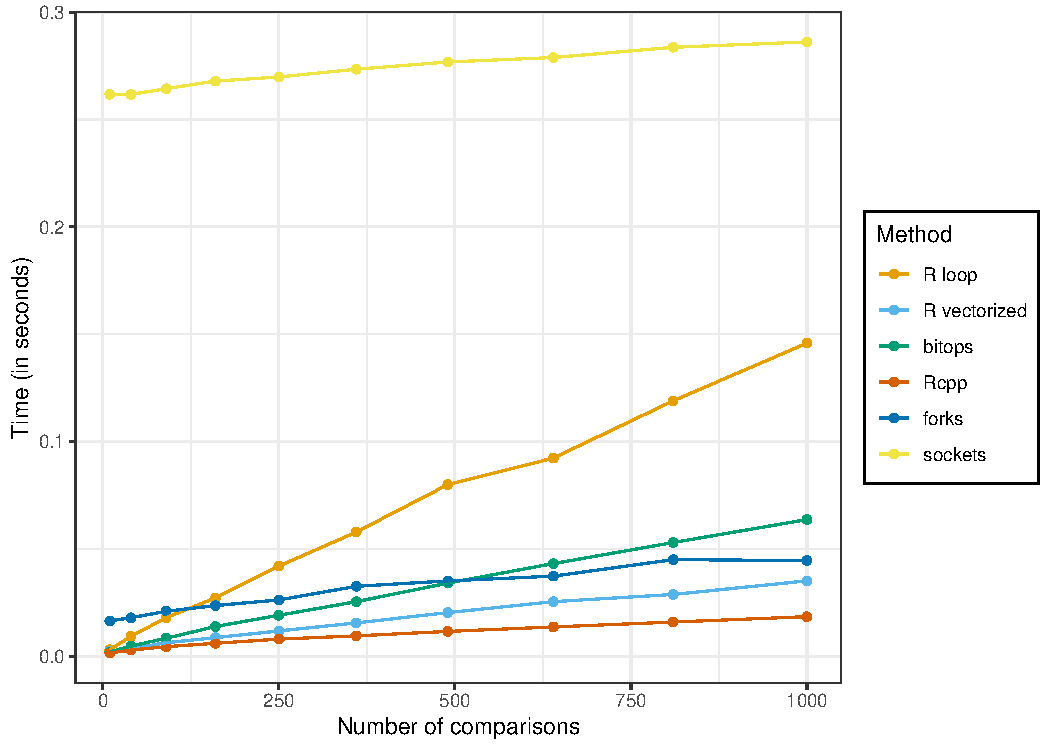
\includegraphics[width=0.8\linewidth]{figure/parallel_plot-1} 

}

\caption[This figure plots the running time in seconds against the number of fingerprint-comparisons for each Tanimoto similarity function defined in this paper]{This figure plots the running time in seconds against the number of fingerprint-comparisons for each Tanimoto similarity function defined in this paper.}\label{fig:parallel_plot}
\end{figure}

\end{knitrout}

To conclude this paper, we will fit linear and quadratic models to the running times in Figure \ref{fig:parallel_plot}. Table \ref{tab:model_run_time} presents the $R^2$ values obtained. We observe that the $R^2$ values for all models are large, and the differences in $R^2$ between the linear and quadratic models are very small. Therefore, the results in Table \ref{tab:model_run_time}, together with Figure \ref{fig:parallel_plot}, indicate that the complexity of all functions is linear. Of course, the rate at which the running times increase with the number of comparisons is different for each method (see Figure \ref{fig:parallel_plot}). 

\begin{knitrout}
\definecolor{shadecolor}{rgb}{0.969, 0.969, 0.969}\color{fgcolor}\begin{kframe}
\begin{alltt}
\hldef{linear_models} \hlkwb{<-} \hlkwd{tapply}\hldef{(}
  \hlkwc{X} \hldef{= df_times,}
  \hlkwc{INDEX} \hldef{= df_times}\hlopt{$}\hldef{expr,}
  \hlkwc{FUN} \hldef{=} \hlkwa{function}\hldef{(}\hlkwc{x}\hldef{)} \hlkwd{lm}\hldef{(time} \hlopt{~} \hldef{comparisons,} \hlkwc{data} \hldef{= x)}
\hldef{)}
\hldef{R2_linear} \hlkwb{<-} \hlkwd{sapply}\hldef{(linear_models,} \hlkwc{FUN} \hldef{=} \hlkwa{function}\hldef{(}\hlkwc{x}\hldef{)} \hlkwd{summary}\hldef{(x)}\hlopt{$}\hldef{r.squared)}

\hldef{quadratic_models} \hlkwb{<-} \hlkwd{tapply}\hldef{(}
  \hlkwc{X} \hldef{= df_times,}
  \hlkwc{INDEX} \hldef{= df_times}\hlopt{$}\hldef{expr,}
  \hlkwc{FUN} \hldef{=} \hlkwa{function}\hldef{(}\hlkwc{x}\hldef{)} \hlkwd{lm}\hldef{(time} \hlopt{~} \hldef{comparisons} \hlopt{+} \hlkwd{I}\hldef{(comparisons}\hlopt{^}\hlnum{2}\hldef{),} \hlkwc{data} \hldef{= x)}
\hldef{)}
\hldef{R2_quad} \hlkwb{<-} \hlkwd{sapply}\hldef{(quadratic_models,} \hlkwc{FUN} \hldef{=} \hlkwa{function}\hldef{(}\hlkwc{x}\hldef{)} \hlkwd{summary}\hldef{(x)}\hlopt{$}\hldef{r.squared)}

\hlkwd{rbind}\hldef{(}
  \hlsng{"Linear"} \hldef{= R2_linear,}
  \hlsng{"Quadratic"} \hldef{= R2_quad}
\hldef{)} \hlopt
  \hlkwd{kbl}\hldef{(}
    \hlkwc{digits} \hldef{=} \hlnum{3}\hldef{,}
    \hlkwc{format} \hldef{=} \hlsng{"latex"}\hldef{,}
    \hlkwc{booktabs} \hldef{=} \hlnum{TRUE}\hldef{,}
    \hlkwc{linesep} \hldef{=} \hlsng{""}\hldef{,}
    \hlkwc{table.envir} \hldef{=} \hlsng{"table\} \textbackslash{}\textbackslash{}captionsetup\{margin = 60pt"}\hldef{,}
    \hlkwc{caption} \hldef{=} \hlkwd{paste0}\hldef{(}\hlsng{"$R^2$ values for the linear and quadratic model "}\hldef{,}
                     \hlsng{"regressing running time (in seconds) on the "}\hldef{,}
                     \hlsng{"number of comparisons made for each of the "}\hldef{,}
                     \hlsng{"methods as used in the figure above."}\hldef{)}
  \hldef{)} \hlopt
  \hlkwd{kable_styling}\hldef{(}\hlkwc{latex_options} \hldef{=} \hlkwd{c}\hldef{(}\hlsng{"HOLD_position"}\hldef{))}
\end{alltt}
\end{kframe}\begin{table}[H] \captionsetup{margin = 60pt}
\centering
\caption{\label{tab:model_run_time}$R^2$ values for the linear and quadratic model regressing running time (in seconds) on the number of comparisons made for each of the methods as used in the figure above.}
\centering
\begin{tabular}[t]{lrrrrrr}
\toprule
  & R loop & R vectorized & bitops & Rcpp & forks & sockets\\
\midrule
Linear & 0.997 & 0.993 & 0.998 & 0.980 & 0.956 & 0.976\\
Quadratic & 0.998 & 0.998 & 1.000 & 0.995 & 0.987 & 0.995\\
\bottomrule
\end{tabular}
\end{table} \captionsetup{margin = 60pt}

\end{knitrout}





\end{enumerate}

\end{document}


